%header and footer for separate chapter files

\ifx\whole\undefined
\documentclass[12pt, leqno]{book}
\usepackage{graphicx}
\input style-for-curves.sty
\usepackage{hyperref}
\usepackage{showkeys} %This shows the labels.
%\usepackage{SLAG,msribib,local}
%\usepackage{amsmath,amscd,amsthm,amssymb,amsxtra,latexsym,epsfig,epic,graphics}
%\usepackage[matrix,arrow,curve]{xy}
%\usepackage{graphicx}
%\usepackage{diagrams}
%
%%\usepackage{amsrefs}
%%%%%%%%%%%%%%%%%%%%%%%%%%%%%%%%%%%%%%%%%%
%%\textwidth16cm
%%\textheight20cm
%%\topmargin-2cm
%\oddsidemargin.8cm
%\evensidemargin1cm
%
%%%%%%Definitions
%\input preamble.tex
%\input style-for-curves.sty
%\def\TU{{\bf U}}
%\def\AA{{\mathbb A}}
%\def\BB{{\mathbb B}}
%\def\CC{{\mathbb C}}
%\def\QQ{{\mathbb Q}}
%\def\RR{{\mathbb R}}
%\def\facet{{\bf facet}}
%\def\image{{\rm image}}
%\def\cE{{\cal E}}
%\def\cF{{\cal F}}
%\def\cG{{\cal G}}
%\def\cH{{\cal H}}
%\def\cHom{{{\cal H}om}}
%\def\h{{\rm h}}
% \def\bs{{Boij-S\"oderberg{} }}
%
%\makeatletter
%\def\Ddots{\mathinner{\mkern1mu\raise\p@
%\vbox{\kern7\p@\hbox{.}}\mkern2mu
%\raise4\p@\hbox{.}\mkern2mu\raise7\p@\hbox{.}\mkern1mu}}
%\makeatother

%%
%\pagestyle{myheadings}

%\input style-for-curves.tex
%\documentclass{cambridge7A}
%\usepackage{hatcher_revised} 
%\usepackage{3264}
   
\errorcontextlines=1000
%\usepackage{makeidx}
\let\see\relax
\usepackage{makeidx}
\makeindex
% \index{word} in the doc; \index{variety!algebraic} gives variety, algebraic
% PUT a % after each \index{***}

\overfullrule=5pt
\catcode`\@\active
\def@{\mskip1.5mu} %produce a small space in math with an @

\title{Personalities of Curves}
\author{\copyright David Eisenbud and Joe Harris}
%%\includeonly{%
%0-intro,01-ChowRingDogma,02-FirstExamples,03-Grassmannians,04-GeneralGrassmannians
%,05-VectorBundlesAndChernClasses,06-LinesOnHypersurfaces,07-SingularElementsOfLinearSeries,
%08-ParameterSpaces,
%bib
%}

\date{\today}
%%\date{}
%\title{Curves}
%%{\normalsize ***Preliminary Version***}} 
%\author{David Eisenbud and Joe Harris }
%
%\begin{document}

\begin{document}
\maketitle

\pagenumbering{roman}
\setcounter{page}{5}
%\begin{5}
%\end{5}
\pagenumbering{arabic}
\tableofcontents
\fi



\chapter{Appendix: Syzygies and Geometry}\label{syzygy chapter}

\section{Betti tables}

 In this Chapter we will return to the case of standard graded rings $R$; that is, $R$ is an algebra over the field $k := R_0$, and is generated by the finite dimensional vector space $R_1$. In particular, $R$ is a homomorphic image of 
$S = k[R_1]$, and thus $R$ is Noetherian. Throughout this section, $S$ will denote a standard graded polynomial ring.

A module over any ring can be specified by its generators and relations. But Hilbert saw that there was something to be gained by studying the relation on the relations, and the relations on those, and so on---in short, the syzygies of the module.
In the case of a graded module $M$ over a graded ring $R$, we may take a minimal free resolution
$$
0\lTo M \lTo F_0 \lTo^{d_{1}} F_1\lTo^{d_{2}}\cdots
$$
that is graded, with differential $d$ of degree 0. The $i$-th syzygy module of M is by definition the 
cokernel of $d_{i+1}$. Recall that $R(-a)$ denotes a rank one free graded module generated in degree $a$ (so that $R(-a)_0 = R_a$ and more generally $R(a)_{b} = R_{a+b}$). We may identify each $F_i$ with a direct sum of the form 
$\bigoplus_j R(-a_j)^{\gb_{i,j}}$
in such a way that the homomorphisms $d_{i}$ are homogeneous of degree 0. 
Theorem~\ref{uniqueness} holds in this case as well, so that 
the numbers $\beta_{i,j}$ depend only on the module $M$, as is also obvious from the formula $\Tor_i(M,k) = \bigoplus_j k(-a_j)^{\gb_{i,j}}$.
We sometimes refer to $\beta_{i,j}$ informally as the \emph{number of $i$-th syzygies of degree $j$}; more properly, it is the number of minimal generators of degree $j$ required by the module of $i$-th syzygies of $M$.

For convenience, the graded Betti numbers are usually displayed in a compact \emph{Betti table}, with the nonzero $\beta_{i,j}$ appearing in the $i$-th column and the $(j-i)$-th row: \footnote{The reason for the initially non-intuitive choice $j-i$ instead of $j$ is that, for the resolution $\FF$ to be minimal, it is necessary that if $\beta_{i,j}\neq 0$, then some $\beta_{i-1,k}\neq 0$ for some $k<j$. Thus shift by $-j$ makes the diagram more compact.) This useful convention goes back to the development of the program Macaulay by Dave Bayer and Mike Stillman  in the 1980s. In those days of small displays, efficiency was even more important than now.}
%\setcounter{MaxMatrixCols}{13}
%\begin{small}
%$$
%\begin{matrix}
%j \backslash i     &0&1&2&3&4&5&6&7&8&9&10&11\\ \hline
%%\text{total:}&1&55&359&1211&2602&3824&3954&2889&1466&493&99&9 \\
%\text{0: }\vline &1&.&\text{.}&\text{.}&\text{.}&\text{.}&\text{.}&\text{.}&\text{.}&\text{.}&\text{.}&\text{.}\\
%\text{1: }\vline &.&55&320&930&1688&2060&1728&987&368&81&8&\text{.}\\
%\text{2: }\vline &\text{.}&\text{.}&39&280&906&1736&2170&1832&1042&384&83&8\\
%\text{3: }\vline &\text{.}&\text{.}&\text{.}&1&8&28&56&70&56&28&8&1\\
%\end{matrix}
%$$
%\end{small}
\setcounter{MaxMatrixCols}{13}
\begin{small}
$$
\begin{matrix}
j \backslash i     &0&1&2\\ \hline
%\text{total:}&1&55&359&1211&2602&3824&3954&2889&1466&493&99&9 \\
\text{0 }\vline &\gb_{0,0}&\gb_{1,1}&\gb_{2,2}&\cdots&\\
\text{1 }\vline &\gb_{0,1}&\gb_{1,2}&\gb_{2,3}&\cdots&\\
\text{2 }\vline &\gb_{0,2}&\gb_{1,3}&\gb_{2,4}&\cdots&\\
\vdots&\vdots&\vdots&\cdots&\\
%\text{3: }\vline &\text{.}&\text{.}&\text{.}&1&8&28&56&70&56&28&8&1\\
\end{matrix}
$$
\end{small}
\noindent For the sake of simplicity we usually replace some 0 entries with $-$.
We sometimes speak of the \emph{Betti table of a module $M$}, by which we mean the Betti table of the minimal free resolution
of $M$. Similarly, when we speak of the Betti table of a variety $X\subset \PP^{n}$, we mean the Betti table of the minimal free resolution
of the homogeneous coordinate ring $S_{X}$ of $X$, as a module over the homogeneous coordinate ring of $\PP^{n}.$ 

The rows of the betti table correspond to \emph{linear strands} of the resolution---sequences of the free summands where the maps between them are represented by matrices of linear forms. The length of the linear strands plays a central role in Green's conjecture. 


\section{Which tables are Betti tables of minimal resolutions?}\label{which tables}
Here are some ideas that can help with the computation of Betti tables. The fact that minimal free resolutions are
constructed by successively choosing minimal sets of generators for the kernel of a previously 
computed map leads to this:

\begin{proposition}\label{zero implications}
Supoose that $\beta_{i,j}$ are the graded Betti numbers of an $S$-module. If $\beta_{i_{0},i_{0}+j} = 0$ for all $j\leq j_{0}$  then
$\beta_{i, i+j} = 0$ for all $i\geq i_{0},\ j\leq j_{0}$ as illustrated in Figure ~\ref{17.2.1}.
\end{proposition}
\begin{figure}[ht!]
\centering
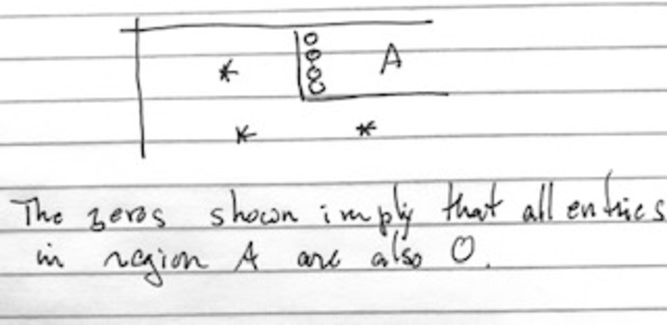
\includegraphics[width=90mm]{illust-17-2-1.pdf}
\caption{The zeros shown imply that all entries in region A are also 0.\label{17.2.1}}
\end{figure}
Note that $\beta_{i,j}$ and $\beta_{i+1,j+1}$ are consecutive elements of the same row of the Betti
table, so the Proposition says that a zero entry in the $i$-position of all the rows of the table at and above
a certain spot implies that all successive entries
of those rows are zero as well.

\begin{proof}
The table represents the summands of a minimal free resolution, and minimality means that the maps in the resolution are represented by matrices whose entries have strictly positive degree. Thus if
$F_{i}$ has no summand isomorphic to $S(-j)$ for $j\leq j_{0}$ it follows that there can be no summand
of $F_{i+1}$ isomorphis to $S(-j-1)$ for the same range of $j$.
\end{proof}

 Hilbert's original application of the Syzygy Theorem was to compute the Hilbert function of a module as a (finite!) alternating sum of the (easy to compute) Hilbert functions of the free modules in the resolution. If the graded Betti numbers of $M$ are $\{\beta_{i,j}\}$, then clearly
\begin{align*}
 H_{M}(t) &= \sum_{i}(-1)^{i}\sum_{j}\beta_{i,j}H_{S(-j-i)}\\
 &= \sum_{i}(-1)^{i}\sum_{j}\beta_{i,j}{n-j+t\choose n}
\end{align*}
Reversing the order of summation, we note that $H_{M}(t)$ can be computed from the Betti table as the 
alternating sum, with appropriate binomial coefficients, of the $t$-th anti-diagonal of the Betti table. 

Suppose now that the Hilbert function $H_{M}(t)$ of a finitely generated
graded module $M$ is known, and that we are interested in understanding the Betti table of the module's minimal resolution. To simplify the notation, set $m_{t} := H_{M}(t)$. Since the Hilbert function of the residue field $k$ has values $(1,0,0,\dots)$, and the $S$-free resolution of $k$ is the
Koszul complex $\KK$, with Betti table
$$
\begin{matrix}
j \backslash i     &0&1&2\\ \hline
%\text{total:}&1&55&359&1211&2602&3824&3954&2889&1466&493&99&9 \\
\text{0 }\vline &1&n+1&{n+1\choose 2}&\dots\\
\text{1 }\vline &-&-&-&\dots\\
\end{matrix},
$$
we can produce a (generally not finitely generated) module 
$$
M' := \bigoplus_{-N}^{\infty}k(-t)^{m_{t}}
$$
with the same Hilbert function, and resolution a corresponding direct sum of shifted Koszul complexes. 
A priori this tells us nothing about the Betti table of $M$. However,
there is a flat deformation $\sM$ over $k[z]$ of the module $M$ to the trivial module 
$\oplus_{t}k(-t)^{m_{t}}$
obtained by pulling back $M$ along the map
$$
k[x_{0}\dots,x_{n}] \to k[x_{0},\dots,x_{n}]: \quad x_{i} \mapsto zx_{i}
$$
and taking the flat limit at $z=0$. 
The Betti table of the fiber of $\sM$ over $z=0$ is thus
\begin{align*}
B_{0} =  \begin{matrix}
j \backslash i     &0&1&2\\ \hline
%\text{total:}&1&55&359&1211&2602&3824&3954&2889&1466&493&99&9 \\
\text{\kern 5pt t-1}\vline &\cdots&\cdots&\cdots&\cdots\\
\text{ \kern 7pt t }\vline &m_{t}&m_{t}(n+1)&m_{t}{n+1\choose 2}&\dots\\
\text{t+1}\vline &m_{t+1}&m_{t+1}(n+1)&m_{t+1}{n+1\choose 2}&\dots\\
\text{t+2}\vline &\cdots&\cdots&\cdots&\cdots\\
\end{matrix}
\end{align*}
Such a flat deformation corresponds to a deformation of resolutions, as well, and one may deduce:

\begin{proposition}\cite{Peeva}\label{cancellation}
With notation as above, the Betti table $B$ of $M$ is obtained from the array $B_{0}$ by successively cancelling pairs of terms along the anti-diagonals; that is $B$ is derived from $B_{0}$ by repeated moves of the form
\begin{align*}
\begin{matrix}
j \backslash i     &j-1&j&j+1\\ \hline
%\text{total:}&1&55&359&1211&2602&3824&3954&2889&1466&493&99&9 \\
\text{\kern 19pt}\vline &\cdots&\cdots&\cdots&\cdots\\
\text{ \kern 7pt t }\vline &\dots&\dots&b&\dots\\
\text{t+1}\vline &\dots&c&\dots&\dots\\
\text{\kern 19pt}\vline &\cdots&\cdots&\cdots&\cdots\\
\end{matrix}
\quad \mapsto\quad
\begin{matrix}
j \backslash i     &j-1&j&j+1\\ \hline
%\text{total:}&1&55&359&1211&2602&3824&3954&2889&1466&493&99&9 \\
\text{\kern 19pt}\vline &\cdots&\cdots&\cdots&\cdots\\
\text{ \kern 7pt t }\vline &\dots&\dots&b-1&\dots\\
\text{t+1}\vline &\dots&c-1&\dots&\dots\\
\text{\kern 19pt}\vline &\cdots&\cdots&\cdots&\cdots\\
\end{matrix}
\end{align*}
\end{proposition}


\section{Examples of Betti Tables}
Some examples will help absorb these ideas.

%\begin{example}[A point in $\PP^3$]
%Any point in $\PP^3$ is the intersection of 3 hyperplanes, so it has Betti table:
%\begin{small}
%$$
%\begin{matrix}
%j \backslash i &0&1&2&3\\ \hline
%\text{0 }\vline &1&3&3&1\\
%\text{1 }\vline &-&-&-&-\\
%\end{matrix}
%$$
%\end{small}
%Note that the matrices of the differentials in the resolution---the Koszul complex on 3 linear forms---are all linear; again, this is reflect in the fact that all the 
%nonzero entries of the table are on one horizontal line.
%\end{example}

\begin{example}\label{3 points in P2}
As a first example, let $X$ be a set of three non-collinear points in $\PP^2$, say
$X = \{(1,0,0), (0,1,0), (0,0,1)\}$. Since no linear form vanishes on $X$, the Hilbert function of $S_{X}$ begins $1,3$. Since $S_{X}$ is reduced, the multiplication by a general linear form on $S_{X}$ is a monomorphism, so the Hilbert function is non-decreasing and since $\deg X = 3$ it must continue $1,3,3,3,\dots$. The linear form 
$\ell :=x_{0}+x_{1}+x_{2}$ does not vanish on any of the points, so it is a nonzerodivisor on $S_{X}$. By Proposition~\ref{reduction modulo a nzd}, the Betti table of $X$ is the same as that of 
$S_{X}/(\ell)$, regarded as a module over $\overline S := k[x_{0}, x_{1}]$. The Hilbert function of $S_{X}/(\ell)$ is the first difference 
$$
1-0,\ 3-1,\ 3-3,\dots = 1,2,0,\dots
$$
of the Hilbert function of $S_{X}$. Thus the Betti table of $S_{X}$ is the same as that of the square of the maximal ideal in $\overline S$. By Proposition~\ref{cancellation} if must be obtained from the table
\begin{small}
$$
\begin{matrix}
j \backslash i &0&1&2&3\\ \hline
\text{0 }\vline &1&2&1\\
\text{1 }\vline &2&4&2&-\\
\end{matrix}
$$
\end{small}
by successive cancellations along anti-diagonals. Since $I_{X}$ does not contain a linear form, we see from Proposition~\ref{zero implications} that the first row
must become $1,0,0$ after cancellation, and thus the second row becomes
$0,3,2$; that is, the Betti table of $X$ is
\begin{small}
$$
\begin{matrix}
j \backslash i     &0&1&2\\ \hline
%\text{total:}&1&55&359&1211&2602&3824&3954&2889&1466&493&99&9 \\
\text{0 }\vline &1&-&-\\
\text{1 }\vline &-&3&2\\
\text{2 }\vline &-&-&-\\
\end{matrix}
$$
\end{small}
The fact that the 3 and the 2 are on the same line is reflects the fact that the 2 syzygies of the ideal $(x,y)^{2}$ are linear; this is a linear strand of the resolution. 

To check all this, we observe that $I_{X}$ indeed contains the three quadrics $x_{0}x_{1}, x_{0}x_{2}, x_{1}x_{2}$.
Since $ \ell_i(\ell_j\ell_k) = \ell_j(\ell_k\ell_i) = \ell_k(\ell_i\ell_j)$ we also see the
 two linear syzygies among these forms. 
 
 Since we already know the Betti table, we see that the resolution
 of $S_{X}$ must be
$$
0\lTo S/I\lTo S
\lTo^{\begin{pmatrix}
\ell_2\ell_3&\ell_1\ell_3&\ell_1\ell_2
\end{pmatrix}}
 S(-1)^3
 \lTo^{\begin{pmatrix}
  \ell_1&0\\
  -\ell_2&\ell_2\\
 0&-\ell_3
 \end{pmatrix}}
 S(-2)^2
 \lTo 0
$$
\begin{exercise}
Prove that the given complex is a resolution using Theorem~\ref{WMACE}.
\end{exercise}
 
Note that the
ideal $I$ can be written as the ideal of $2\times 2$ minors of the matrix
$$
 {\begin{pmatrix}
  \ell_1&0\\
  -\ell_2&\ell_2\\
 0&-\ell_3
 \end{pmatrix}}.
$$
The resolution above is thus a special case of the Eagon-Northcott complex, described in Chapter~\ref{14- canonical curves}
\end{example}

\begin{example}
 Next, consider the twisted cubic curve $C\subset \PP^{3}$, the image of $\PP^{1}$ under the linear series
 $(s^{3}, s^{2}t, st^{2}, t^{3})\subset H^{0}(\sO_{\PP^{1}}(3))$. Write $S = k[x_{0},\dots,x_{3}]$ for the homogeneous coordinate ring of $\PP^{3}$ and $S_{C} = S/I_{C}$ for the homogeneous coordinate ring of $C$.

As we saw in Chapter ****, the ideal of forms vanishing on the twisted cubic is generated by three quadrics
$q_{1}, q_{2}, q_{3}$ that are the $2\times 2$ minors of the
$$
\phi := \begin{pmatrix}
 x_{0}&x_{1}\\
 x_{1}&x_{2}\\
 x_{2}&x_{3}
\end{pmatrix}.
$$
As discussed in Chapter~\ref{canonical curves} the $S$-free resolution of $S_{C}$ is an Eagon-Northcott complex, in this this case
$$
0 \rTo S^{2}(-3) \rTo^{\phi} S^{3}(-2) \rTo^{
\begin{pmatrix}
q_{1}&q_{2}&q_{3} 
\end{pmatrix}
} S.
$$

Thus the Betti table of the twisted cubic is the same as that of the 3 non-collinear points in $\PP^{2}.$

To understand this from another point of view, note that since $I_{C}$ is a prime ideal, $x_{3}$ (or any variable) is a nonzerodivisor on $S_{C}$. Thus we may apply the following result:

\begin{proposition}\label{reduction modulo a nzd}
Let $R$ be a local or standard graded polynomial ring, and let 
$M$ be an $R$-module with minimal $R$-free resolution $\FF$.
If $f\in R$ is a nonzerodivisor on both $R$ and $M$, then the minimal $\overline R:=R/(f)$-free resolution of
$M/fM = \overline R \otimes_{R}M$ is $\overline R \otimes_{R}\FF$, and the Hilbert function of $M/fM$ is
the first difference of that of $M$:  
$$
H_{M/fM}(t) = H_{M}(t) - H_{M}(t-1).
$$
\end{proposition}
\begin{proof}
 The homology of $\overline R \otimes_{R}\FF$ is $\Tor^{R}(\overline R,M)$, which can also be computed as the homology of the tensor product of $M$ with the $R$-free resolution of $R/(f)$. Since $f$ is a nonzerodivisor on $R$, this is
$$
0\to R(-1)\rTo^{f} R \rTo R/(f) \to 0.
$$
It follows that the homology of $\overline R \otimes_{R}\FF$ is the same as the homology of
$$
(0\to R(-1)\rTo^{f} R)\otimes_{R}M  = 0\to M(-1)\rTo^{f} M.
$$
Since $f$ is a nonzerodivisor on $M$, we see that $H_{i}( \overline R \otimes_{R}\FF) = 0$ for $i>0$, showing that $\overline R \otimes_{R}\FF$
is a free resolution of $M/(f)M$. The minimality is obvious. The formula for the Hilbert functions follows from the same exact sequences.
\end{proof}

Proposition~\ref{reduction modulo a nzd} shows that the minimal free resolution of $C$ has the same Betti table as the minimal free resolution of $S_{C}/(\ell) = S/(I_{c}+(\ell))$ for any linear form $\ell$ and this corresponds to the 
scheme that is the intersection of $C$ with the hyperplane $\ell = 0$. For sufficiently general $\ell$ (or even
for $\ell = x_{0}-x_{3}$)) this consists of three non-colinear points in the plane.

However, this is not quite all that needs to be said: certainly $I_{C}+(x_{3})$ is an ideal defining the hyperplane section $x_{3}= 0$ of $C$, but to conclude from  Proposition~\ref{reduction modulo a nzd} that the Betti table of $C$ is the same as that of the 3 noncolinear points, we need to know that $I_{C}+(x_{3})$ is saturated.

By the Auslander-Buchsbaum formula, the depth of $S_{C}$ is 2---that is, $S_{C}$ is a Cohen-Macaulay ring. It follows that the depth of $S_{C}/(x_{3})$ is 1, and this shows that $I_{c}+(x_{3})$ is a saturated ideal completing the circle of ideas.
\end{example}

\begin{exercise}
 Let $C$ be the nonsingular rational quartic $\PP^{3}$, the image of $\PP^{1}$ under the linear series
 $(s^{4}, s^{3}t, st^{3}, t^{4})\subset H^{0}(\sO_{\PP^{1}}(3))$. Show that the general hyperplane section of $C$  is the intersection of two quadrics, while the ideal of $C$ has just one quadric generator. Conclude that
  that the Betti table of $C$ is not the same as the Betti table of the hyperplane section, and thus that
  $S_{C}$ is not Cohen-Macaulay. (in fact, the Betti table of $S_{C}$ is
\begin{small}
$$
\begin{matrix}
j \backslash i &0&1&2&3\\ \hline
\text{0 }\vline &1&-&-&-\\
\text{1 }\vline &-&1&-&-\\
\text{2 }\vline &-&3&4&1\\
\end{matrix},
$$
\end{small}

\noindent from which we see that the projective dimension of $S_{C}$ is 3, so by the Auslander-Buchsbaum theorem the depth is only 1.)
\end{exercise}

%\begin{example}\label{canonical in P3}
%For example, the minimal free resolution of the homogeneous coordinate ring $S_{C}$ of a canonical curve $C$ of genus 4 in $\PP^{3}$ whose ideal is generated by a quadric $q$ and a cubic $f$, as a module over the homogeneous coordinate ring $S = \CC[x_{0},\dots,x_{3}]$ of $\PP^{3}$, is the Koszul complex
%\small
%$$
%S \lTo^{
%\begin{pmatrix}
%  q& f
%\end{pmatrix}}
%S(-2) \oplus S(-3) \lTo^{
%\begin{pmatrix}
%f\\-q 
%\end{pmatrix}
%}
%S(-5)\lTo 0.
%$$
%\normalsize
%since
%$q$ and $f$ are relatively prime, and thus form a regular sequence
%Thus it has  Betti table:
%
%\setcounter{MaxMatrixCols}{13}
%\begin{small}
%$$
%\begin{matrix}
%j \backslash i     &0&1&2\\ \hline
%%\text{total:}&1&55&359&1211&2602&3824&3954&2889&1466&493&99&9 \\
%\text{0 }\vline &1&-&-\\
%\text{1 }\vline &-&1&-\\
%\text{2 }\vline &-&1&-\\
%\text{3 }\vline &-&-&1\\
%\end{matrix}
%$$
%\end{small}
%\end{example}

\begin{example}
 Consider a set $X$ of 7 points in linearly general position $\PP^3$. 
Castelnuovo's Theorem~\ref{castelnuovo} shows that any 6 points in linearly general position lie on a unique twisted cubic, so the first distinction one might make among sets of 7 points is whether the 7th point lies on the twisted cubic too.

As we saw in \ref{****}, any set of $2n+1$ points in linearly general position in $\PP^{n}$ imposes $2n+1$ conditions on quadrics, so in any case $I_{X}$ requires exactly 3 quadratic minimal generators, $q_{1},q_{2},q_{3}$ and the Hilbert function of $S_{X}$ begins $1,4,7,?$. Since $S_{X}$ is reduced, the Hilbert function is non-decreasing, and since the eventual value must be $\deg X = 7$, the function must be
$1,4,7,7,\dots$, and the ideal contains $20-7 = 13$ cubics. From this information we can work out the whole Betti table, as follows. 

Since any set of points has Cohen-Macaulay homogeneous coordinate ring we can apply Proposition~\ref{reduction moduo nzd} to say that the Betti table of $R := S_{X}/(x_{3})$ is the same as that of $S_{X}$. Write $R = \overline S/I$, where $\overline S = k[x_{0},x_{1},x_{2}]$. The Hilbert function of $R$ is determined by the exact sequence
$$
0\rTo S_{X}(-1)\rTo^{x_{3}} S_{X} \rTo R \rTo 0
$$
as the first difference function of that of $S_{X}$, namely
$$
1 -0, 4-1, 7-4, 7-7,\dots = 1,3,3,0,\dots;
$$
that is, $I$ is generated (not minimally) by the 3 quadrics and a total of 10 cubics. By Propositions~\ref{reduction modulo a nzd} and \ref{cancellation}, the Betti table of $X$ must be obtained by successive cancellations
from the table
\begin{small}
$$
\begin{matrix}
j \backslash i &0&1&2&3\\ \hline
\text{0 }\vline &1&3&3&1\\
\text{1 }\vline &3&9&9&3\\
\text{2 }\vline &3&9&9&3\\
\text{3 }\vline &-&-&-&-\\
\end{matrix}
$$
\end{small}
Moreover, since $X$ is not contained in a hyperplane, the zero-th row, after cancellation, must become
\begin{small}
 $
\begin{matrix}
\text{0 }\vline &1&0&0&0\\
\end{matrix},
$
\end{small}
so we can begin by making this cancellation. We also know that $I_{X}$ has exactly 3 quadratic generators, necessitating another cancellation, and we see that the actual Betti table of $X$ must be obtained by
cancelling from
\begin{small}
$$\leqno{(1)}\qquad\qquad
\begin{matrix}
j \backslash i &0&1&2&3\\ \hline
\text{0 }\vline &1&0&0&0\\
\text{1 }\vline &0&3&8&3\\
\text{2 }\vline &0&9&9&3\\
\text{3 }\vline &-&-&-&-\\
\end{matrix}
$$
\end{small}


Now three general quadrics define a complete intersection of 8 points, and it follows that in the case of 7 general points $q_{1},q_{2},q_{3}$ form a complete intersection with resolution the Koszul complex, having Betti table:
\begin{small}
$$
\begin{matrix}
j \backslash i &0&1&2&3\\ \hline
\text{0 }\vline &1&-&-&-\\
\text{1 }\vline &-&3&-&-\\
\text{2 }\vline &-&-&3&-\\
\text{3 }\vline &-&-&-&1\\
\end{matrix}.
$$
\end{small}
In this case there are no linear relations among $q_{1},q_{2},q_{3}$, so the 8 and 3 in row 1 of table (1) must 
cancel completely, giving
\begin{small}
$$
\begin{matrix}
j \backslash i &0&1&2&3\\ \hline
\text{0 }\vline &1&0&0&0\\
\text{1 }\vline &0&3&0&0\\
\text{2 }\vline &0&1&6&3\\
\text{3 }\vline &-&-&-&-\\
\end{matrix}
$$
\end{small}
Since no further cancellation is possible, this must be the Betti table of a  set $X$ of 7 general points.

On the other hand, if the points lie on a twisted cubic, then $q_{1}, q_{2}, q_{3}$ generate the ideal of the twisted cubic, and as we  see from the Betti table in Example~\ref{}, these have 2 linear relations, which are themselves independent. It follows that row 1 of the Betti table of $X$ must cancel to become 
\begin{small}
 $
\begin{matrix}
\text{1 }\vline &0&3&2&0\\
\end{matrix}.
$
\end{small}
Thus the Betti table of $X$ in this case is
\begin{small}
$$
\begin{matrix}
j \backslash i &0&1&2&3\\ \hline
\text{0 }\vline &1&0&0&0\\
\text{1 }\vline &0&3&2&0\\
\text{2 }\vline &0&7&9&3\\
\text{3 }\vline &-&-&-&-\\
\end{matrix}
$$
\end{small}

\end{example}
Thus the Betti tables detect whether the points lie on a twisted cubic curve.


\section{Interpreting homological ring theory through Betti tables}

Suppose that $R = S/I$ is a  factor ring of codimension $c$ in $S$ and that
$$
\FF: 0 \rTo F_{m} \rTo\cdots\rTo F_{0}
$$ 
is its minimal free resolution. Theorem~\ref{depth} %in Chapter 16
Shows that the dual of $\FF$, which computes $\Ext_{S}(R,S)$, is exact for the $c$ steps beginning
with $F_{0}^{*}$, but has homology at $F_{c}^{*}$:
$$
\FF: 0 \rTo F_{0}^{*} \rTo\cdots\rTo F_{c}^{*} \rTo\cdots.
$$ 
On the other hand, the Auslander-Buchsbaum formula shows that the projective dimension of $R$
as an $S$-module is $\dim S - \depth R$. Taking into account that $\omega_{S} = S(-n-1)$, this proves:
\begin{proposition}
 Let $R = S/I$ be a graded factor ring of the polynomial ring $S$. If $I$ has codimension $c$, then
 $R$ is Cohen-Macaulay if and only if the projective dimension of $R$ is $c$, the smallest possible value.
 In this case the dual of the minimal $S$-free resolution of $R$ is the minimal $S$-free resolution of
 $\omega_{R} := Ext^{c}(R,S(-n-1))$.
\end{proposition}

The Betti table of $\FF^{*}$ is obtained from that of $\FF$ by reversing it left-to-right and top-to-bottom, adjusting the row indices appropriately; for example if $\FF$ is the resolution of the twisted cubic,
(Example~\ref{***}), then the Betti table of $\FF^{*}$, the resolution of the module associated to 
the sheaf $\omega_{C}(4)$, is 
\begin{small}
$$
\begin{matrix}
j \backslash i &0&1&2&3\\ \hline
\text{-3 }\vline &2&3&0&0\\
\text{-2 }\vline &0&0&1&0\\
\text{-1 }\vline &-&-&-&-\\
\end{matrix}
$$
\end{small}

The restriction on the tables that can occur as Betti tables of resolutions given in Proposition~\ref{zero restrictions} is not symmetric under this operation (the other restrictions in Section~\ref{which tables} are). Dualizing it, we get a new restriction on the Betti table of a Cohen-Macaulay factor ring:

\begin{corollary}\label{dual zero restrictions}
 Suppose that $R = S/I$ is a Cohen-Macaulay graded ring with minimal free resolution $\FF$ having
 graded Betti numbers
 $\beta_{i,j}$. If, for some index $i_{0}$ we have $\beta_{i,j} = 0$ for all $j\geq i_{0}+j_{0}$, then
 $\beta_{i,j} = 0$ for all $i,j$ with $i\leq i_{0}$ and $j\geq i+j_{0}$. 
 \end{corollary}
\begin{figure}[ht!]
\centering
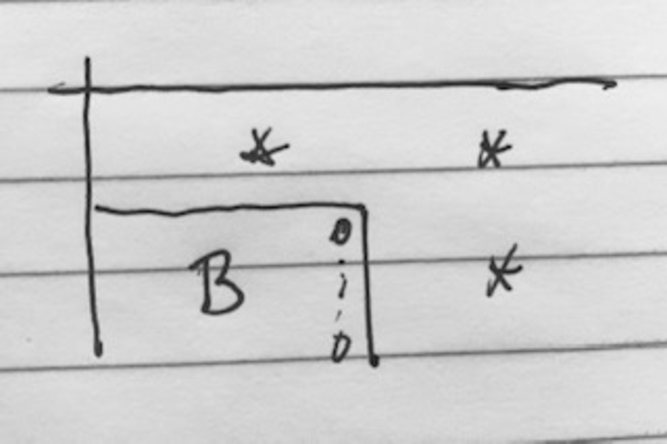
\includegraphics[width=90mm]{illust-17-4-1.pdf}
\caption{In the resolution of a Cohen-Macaulay module, the zeros shown imply that the entries in region B are zero. \label{17.4.1}}
\end{figure}

We can also characterize the condition for $S/I$ to be Gorenstein:

\begin{proposition}\label{Gorenstein characterization}
Suppose that $R = S/I$ is a graded Cohen-Macaulay ring of codimension $c$, with minimal $S$-free resolution 
$\FF$. The following conditions are equivalent:
\begin{enumerate}
 \item $R$ is Gorenstein.
 \item $F_{c} \cong S(-d)$ for some integer $d$.
 \item The Betti table of $R$ is symmetric; it is equal up to shift to the Betti table of $\FF^{*}$.
\end{enumerate}
\end{proposition}

Even the shifts in this duality can be eliminated if we take not $\FF^{*}$ but $\Hom(\FF, \omega_{S})$ 
with $\omega_{S} = S(-n-1)[-n]$, that is, a rank one free module generated in degree $n+1$ whose
homological degree is $n$.

\begin{proof}
 
\end{proof}

\section{Regularity of modules and sheaves}
The number of the last nonzero column of the Betti table of the resolution of a graded $S$-module $M$ is the projective dimension of $M$. The number of the last row is also an important invariant called the (Castelnuovo-Mumford) \emph {regularity} of $M$. More formally,
\begin{definition}
Let $t_{i}(M) = \max \{j \mid \Tor^{S}_{i}(k,M)_{j} \neq 0\}$. The regularity of $M$ is
$$
\max_{i \geq 0} t_{i}(M)-i.
$$
\end{definition}

As defined above, the regularity of $M$ is obviously an upper bound for the degrees of a minimal generating
set of $M$, which is simply $t_{0}(M)$. One reason the regularity is important is that there is a different expression for the regularity in terms that do not seem to involve the generators directly:

\begin{theorem}
 Let $s_{i}(M) = \max\{j \mid H^{i}_{\gm}(M)_{j} \neq 0\}$. The regularity of $M$ is equal to
 $$
\max_{i \geq 0} t_{i}(M)+i.
$$
\end{theorem}

Note the change of sign; see **** for a proof using local duality. The notion of regularity was introduced by Mumford in the study of sheaves, where it has a slightly simpler expression:

\begin{definition}
A $\sF$ be a sheaf on $\PP^{n}$ is \emph{$m$-regular} if $H^{i}(\sF(m-i) = 0$ for all $i>0$. The \emph{regularity} of $\sF$ is the minimal $m$ for which $\sF$ is $m$-regular.
\end{definition}

 Note that the regularity
of the sheaf $\tilde M$ associated to a graded $S$-module $M$ ignores $H^{0}_{\gm}(M)$ and 
$H^{1}_{\gm}(M)$; but otherwise the definitions are related by the translation from local to global
cohomology and, indeed, if $\depth M \geq 2$ then the regularity of
$M$ is equal to the the regularity of the associated sheaf $\tilde M$ . 

Most applications of
regularity involve the following result\cite{Mumford1966}:
\begin{theorem}

Suppose that $\sF$ is a sheaf on $\PP^{n}$. If $\sF$ is $m$-regular, then $\sF$ is $m'$-regular for all $m'\geq m$, and $\sF(m)$ is generated by its global sections.
\end{theorem}

The regularity of a projective variety $X\subset \PP^{n}$ is  defined to be the regularity of the ideal sheaf of $X$. A striking result of Gruson-Lazarsfeld-Peskine~\cite{***} relates this to more elementary notions:

\begin{theorem}\label{GLP}
 Let $C$ be a reduced, irreducible nondegenerate curve of degree $d$ in $\PP^{n}$. The regularity of $C$ is $\leq d-n+2$, with equality if and only if $C$ is smooth and rational and either $d=n$ or $d=n+1$ or $C$ has a $d-n+3$-secant line. 
 \end{theorem}
 
To see the relevance of the last condition, note that if $C$ has a $d-n+3$-secant line any function
of degree $d-n+2$ that vanishes on $C$ vanishes on the secant line as well; so the ideal of $I_{C}$ of $C$
must require generators of degree at least $d-n+1$. Since the regularity is an upper bound for the degrees of the minimal generators of the ideal of $C$, it follows from the Theorem that $I_{C}$ is generated by
forms of degree $\leq d-n+1$, and we see that the Theorem is sharp in this case. A curve
of degree $d$ with a $d-n+2$-secant is rational, since projection from the line is an isomorphism with $\PP^{1}$.

For a  treatment of these ideas, see for example~\cite{geomsyz}.

\fix{Revised to here 12-5-2020}
\section{Maximal cancellation and the minimal resolution conjecture}
Voisin's Theorem~\ref{} (Green's conjecture) for canonical embeddings of general curves may be interpreted
as saying that all possible cancellations actually occur in that case. Larson's Theorem~\ref{}
\fix{where should Larson's theorem go?} is  statement of the same kind for general linear series of
given degree and dimension on general curves of given genus. 

It would thus seem reasonable to conjecture that such cancellations happen more generally. However, this fails in some cases. Perhaps the simplest example is that of the general projection into $\PP^{6}$ of
an elliptic normal curve of degree 9, whose ideal has Betti table

Perhaps the simplest example is that of a general elliptic curve of degree 9 in $\PP^{6}$
has Betti table
%the following should be aligned in the print version with the 2 directly under the 24. The following produces the correct effect 
%on my screen:
\begin{verbatim}
         2:  12 24 12  . . .
         3:   . 2  16 20 8 1
\end{verbatim}
Such examples were discovered, even for linearly normal curves, by Green and Lazarsfeld~\cite{Green-Lazarsfeld1} and Schreyer (unpublished). 

In 1993 Lorenzini formulated the conjecture that maximal cancellation would hold for the
Betti tables of general sets of points.
One can of course derive examples of sets of points that do not have this property by taking hyperplane sections of the curves above, but these are not general sets of points. However, even for general points, the conjecture fails. The first example, discovered by
Schreyer, is that of $11$ general points in $\PP^{6}$, which has Betti table
 %The 1 should be directly under the 45, and the 25 should be under the 5.
\begin{verbatim}
         2:  17 46 45  5  . .
         3:   .  . 1  25 18 4
\end{verbatim}
 See 
@article {MR1894365,
    AUTHOR = {Eisenbud, David and Popescu, Sorin and Schreyer, Frank-Olaf
              and Walter, Charles},
     TITLE = {Exterior algebra methods for the minimal resolution
              conjecture},
   JOURNAL = {Duke Math. J.},
  FJOURNAL = {Duke Mathematical Journal},
    VOLUME = {112},
      YEAR = {2002},
    NUMBER = {2},
     PAGES = {379--395},
      ISSN = {0012-7094},
   MRCLASS = {13D02 (14M05 15A75)},
  MRNUMBER = {1894365},
MRREVIEWER = {Martin Kreuzer},
       DOI = {10.1215/S0012-9074-02-11226-5},
       URL = {https://doi-org.libproxy.berkeley.edu/10.1215/S0012-9074-02-11226-5},
}
for what seems still to be the state of knowledge about counterexamples for general sets of points, as of this writing. 

Any set of points $X\subset \PP^{n}$ defines a Cohen-Macaulay ring, so the Betti table will not change
if we pass to $A := S_{X}/\ell$ for a general linear form $\ell$, now regarded as a module over a factor ring in
$n$ variables. Since $X$ imposes independent conditions on forms of every degree, it is easy to show
that, if the lowest degree of a generator of the ideal defining $A$ is $d-1$, then the ideal contains the $d$-th power of the ideal of all the variables. But again, this is not a general ideal of that type. It seems that there is no known counterexample to the ``minimal resolution conjecture'' for ideals of the form
$$
J_{V}:= (x_{1},\dots,x_{n})^{d}+V \subset k[x_{1}, \dots, x_{n}]
$$
for a general linear subspace V of the forms of degree $d+1$; more formally, this would say:

\begin{conjecture}[0-dimensional version of the minimal resolution conjecture]
 In the minimal free resolution of an ideal $J_{V}$ as above maximal cancellation holds; that is, there is no index $i$ such that both $\beta_{i,d+i}$ and $\beta_{i+1,d+i}$ are both nonzero.
\end{conjecture}

\section{Boij-Soederberg Theory}
There are further, more subtle restrictions on the form of a Betti table. Since the Betti table of the direct sum of two modules is the sum of the Betti tables of the modules, 
the set of Betti tables of graded modules over a polynomial ring in $n+1$ variables forms a submonoid of 
$\ZZ^{n+2} \times \ZZ^{\infty}$. This monoid is not saturated; for example, 
\begin{small}
$$
B := \begin{matrix}
j \backslash i &0&1&2&3\\ \hline
\text{0 }\vline &1&2&0&0\\
\text{1 }\vline &-&-&2&1\\
\end{matrix}
$$
\end{small}
is not the Betti table of a module, because the top row indicates a map $S^{2}(-1) \to S$, and such
a map must have a linear kernel $S^{1}(-2)$. However, the minimal resolution of the cokernel
of a generic $2\times 4$ matrix has Betti table
\begin{small}
$$
2B := \begin{matrix}
j \backslash i &0&1&2&3\\ \hline
\text{0 }\vline &2&4&-&-\\
\text{1 }\vline &-&-&4&2\\
\end{matrix}.
$$
\end{small}
Finding generators for the monoid of Betti tables is an open problem except in a few small cases (see for example~\cite{Erman-semigroup}. But the cone generated by the Betti tables is known: it is locally simplicial, and there is a simple formula for the extremal rays, as well as a greedy algorithm for writing any Betti table as a sum of rational multiples of the extremal rays. This is the subject of Boij-Soederberg theory. See~\cite{Eisenbud-SchreyerBetti} for more details.

\section{Embeddings of high degree}
\fix{This section is a digression; could go nearly anywhere}

There is a certain uniformity of behavior of  embedded by ``complete linear series associated to line bundles that are sufficiently positive''. Often ``sufficiently positive'' for a line bundle $\sL$ is is taken to mean that
$\sL \otimes \omega_{X}^{-1}$ is a sufficiently high multiple of an ample line bundle. See \cite{LazarsfeldPositivity} for more information. Here is a simple avatar of such results:

\begin{fact}
 Let $X\subset \PP^{n}$ be a variety of dimension $d$, and let $X'\subset \PP^{N} = \PP(H^{0}(\sO_{X}(r))$ be the image of
 $X$ under the $r$-th Veronese mapping. For all $r\gg 0$ the ideal $I_X$ is generated in degree 2,
 and the Betti table of $I_{X}$ has nonzero entries at most in the $d+2$ rows $2,3,\dots,d+3$. Moreover, if 
 $X$ is a set of points in general position, then the Betti table of $X$ has at most 2 nonzero rows.
\end{fact}

\begin{exercise}
Prove the part of the the statement above proven by Mumford in \cite{quadrics}:
\begin{enumerate}

 \item The ideal of the $r$-th Veronese image of $\PP^{n}$  in $\PP^{{n+r\choose n}-1}$
 is generated by the $2\times 2$ minors 
 of the matrix associated to the multiplication map 
 $$
 H^{0}(\sO_{\PP^{n}}(1) \otimes H^{0}(\sO_{\PP^{n}}(r-1) \to  H^{0}(\sO_{\PP^{n}}(r)
 $$
 (see Theorem~\ref{} %in the scrolls chapter
 for this construction).
 
 \item  if $r\gg 0$ then the homogeneous ideal of $X'\subset \PP^{N}$ is generated by the
 ideal of the Veronese image of $\PP^{n}$ together with linear forms.
\end{enumerate}
\end{exercise}

%footer for separate chapter files

\ifx\whole\undefined
%\makeatletter\def\@biblabel#1{#1]}\makeatother
\makeatletter \def\@biblabel#1{\ignorespaces} \makeatother
\bibliographystyle{msribib}
\bibliography{slag}

%%%% EXPLANATIONS:

% f and n
% some authors have all works collected at the end

\begingroup
%\catcode`\^\active
%if ^ is followed by 
% 1:  print f, gobble the following ^ and the next character
% 0:  print n, gobble the following ^
% any other letter: normal subscript
%\makeatletter
%\def^#1{\ifx1#1f\expandafter\@gobbletwo\else
%        \ifx0#1n\expandafter\expandafter\expandafter\@gobble
%        \else\sp{#1}\fi\fi}
%\makeatother
\let\moreadhoc\relax
\def\indexintro{%An author's cited works appear at the end of the
%author's entry; for conventions
%see the List of Citations on page~\pageref{loc}.  
%\smallbreak\noindent
%The letter `f' after a page number indicates a figure, `n' a footnote.
}
\printindex[gen]
\endgroup % end of \catcode
%requires makeindex
\end{document}
\else
\fi

